\newpage
\section{Structure générale et principe}

On a divisé le système en 5 étages avec des interfaces définies.
Le but de la structure choisie est de faciliter le développement et la testabilité
du sous-système, sans avoir besoin du système entier et fonctionnel.

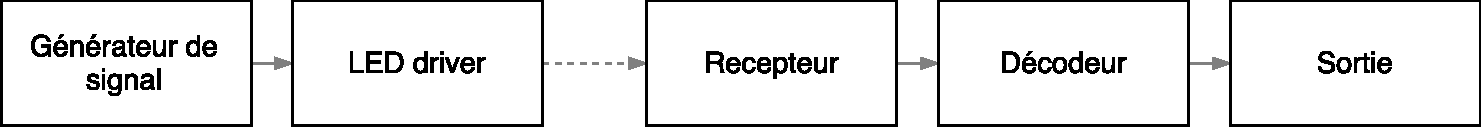
\includegraphics[width=0.8\textwidth]{fig/IRemote_schema_structure}

\subsection{Générateur de signal}

\subsection{LED driver}

\subsection{Récepteur et filtrage}

\subsection{Décodeur}
Le décodeur à 3 fonctions:
\begin{itemize}
	\item{Le comptage des pulses assuré par le \emph{decounter}. Celui-ci signal en \emph{active high} si $n_{pulse}$ ont été reçus par la tension d'entrée depuis son dernier \emph{reset}.}
	\item{La détection de pulse manquant assuré par le \emph{missing pulse detector}. Celui-ci signal en \emph{active low} si la tension d'entrée est maintenue \emph{low} pendant au moins $t_{miss} = xxx \si{\milli\second}$ après la fin d'un pulse.}
	\item{La génération du signal sortant assuré par un délais et des portes logiques. Celui si génère en \emph{active high} un pulse de $t_{true} = xx\si{\milli\second}$ si la salve est \textemp{correcte}.}
\end{itemize}

Une salve est considéré correcte si le \emph{missing pulse }
\begin{center}
	\begin{tabular}{| m{4cm} | m{4cm} | l |}
		\hline
	\thead{\emph{Missing pulse detector}} & \thead{\emph{Decounter}} & \thead{Statu}} & \thead{Sortie}}\ \hline
		low		& low		& Nombre incorrect de pulses dans la salve & low \\ \hline
		low		& high	& Salve correcte	& high\\ \hline
		high	& low		& Salve non finie & low \\ \hline
		high	& high	& Salve non finie & low \\ \hline
	\end{tabular}
\end{center}

\subsection{Sortie}
